% This file was created with tikzplotlib v0.9.15.
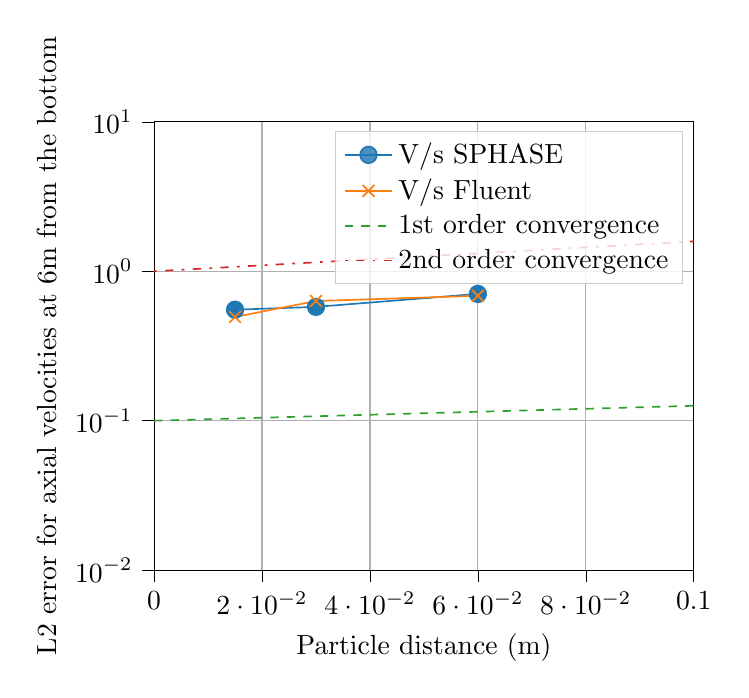
\begin{tikzpicture}

\definecolor{color0}{rgb}{0.12156862745098,0.466666666666667,0.705882352941177}
\definecolor{color1}{rgb}{1,0.498039215686275,0.0549019607843137}
\definecolor{color2}{rgb}{0.172549019607843,0.627450980392157,0.172549019607843}
\definecolor{color3}{rgb}{0.83921568627451,0.152941176470588,0.156862745098039}

\begin{axis}[
legend cell align={left},
legend style={fill opacity=0.8, draw opacity=1, text opacity=1, draw=white!80!black},
log basis y={10},
tick align=outside,
tick pos=left,
x grid style={white!69.0196078431373!black},
xlabel={Particle distance (m)},
xmajorgrids,
xmin=0, xmax=0.1,
xminorgrids,
xtick style={color=black},
y grid style={white!69.0196078431373!black},
ylabel={L2 error for axial velocities at 6m from the bottom },
ymajorgrids,
ymin=0.01, ymax=10,
yminorgrids,
ymode=log,
ytick style={color=black},
ytick={0.001,0.01,0.1,1,10,100},
yticklabels={
  \(\displaystyle {10^{-3}}\),
  \(\displaystyle {10^{-2}}\),
  \(\displaystyle {10^{-1}}\),
  \(\displaystyle {10^{0}}\),
  \(\displaystyle {10^{1}}\),
  \(\displaystyle {10^{2}}\)
}
]
\addplot [semithick, color0, mark=*, mark size=3, mark options={solid}]
table {%
0.015 0.552972072412394
0.03 0.577786216768003
0.06 0.705959538088463
};
\addlegendentry{V/s SPHASE}
\addplot [semithick, color1, mark=x, mark size=3, mark options={solid}]
table {%
0.015 0.494600583856716
0.03 0.632566496807329
0.06 0.685679125768276
};
\addlegendentry{V/s Fluent}
\addplot [semithick, color2, dashed]
table {%
0 0.1
0.1 0.125892541179417
};
\addlegendentry{1st order convergence}
\addplot [semithick, color3, dash pattern=on 1pt off 3pt on 3pt off 3pt]
table {%
0 1
0.1 1.58489319246111
};
\addlegendentry{2nd order convergence}
\end{axis}

\end{tikzpicture}
